\begin{figure}[t]
	\centering
	\begin{subfigure}{0.32\linewidth}
		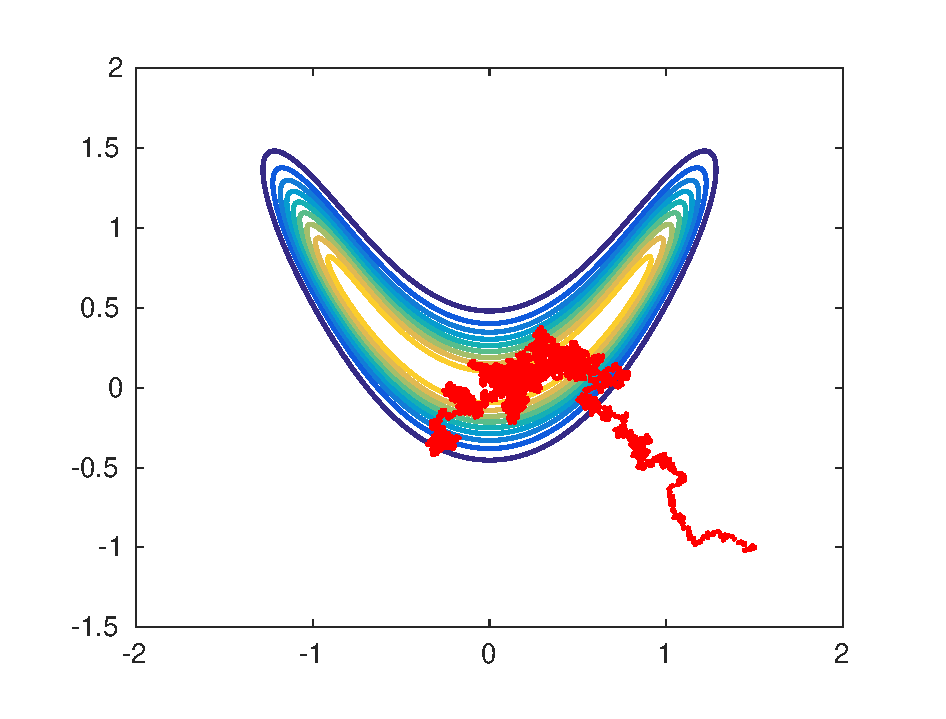
\includegraphics[width=1\linewidth]{plots/MHvsRAM/MH_small}
	\end{subfigure}
	\begin{subfigure}{0.32\linewidth}
		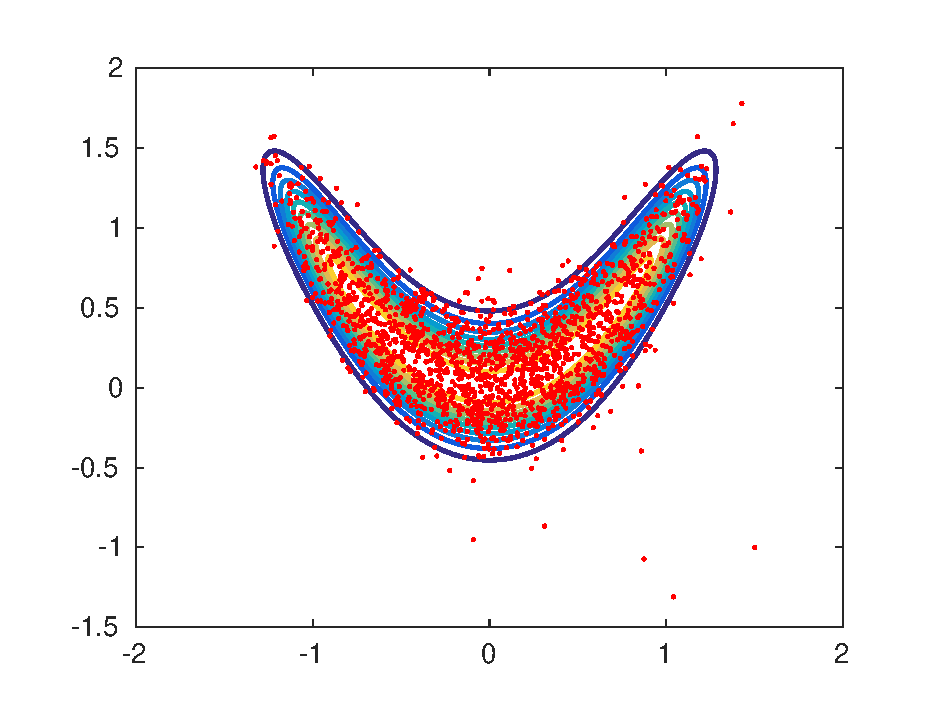
\includegraphics[width=1\linewidth]{plots/MHvsRAM/MH_medium}
	\end{subfigure}
	\begin{subfigure}{0.32\linewidth}
		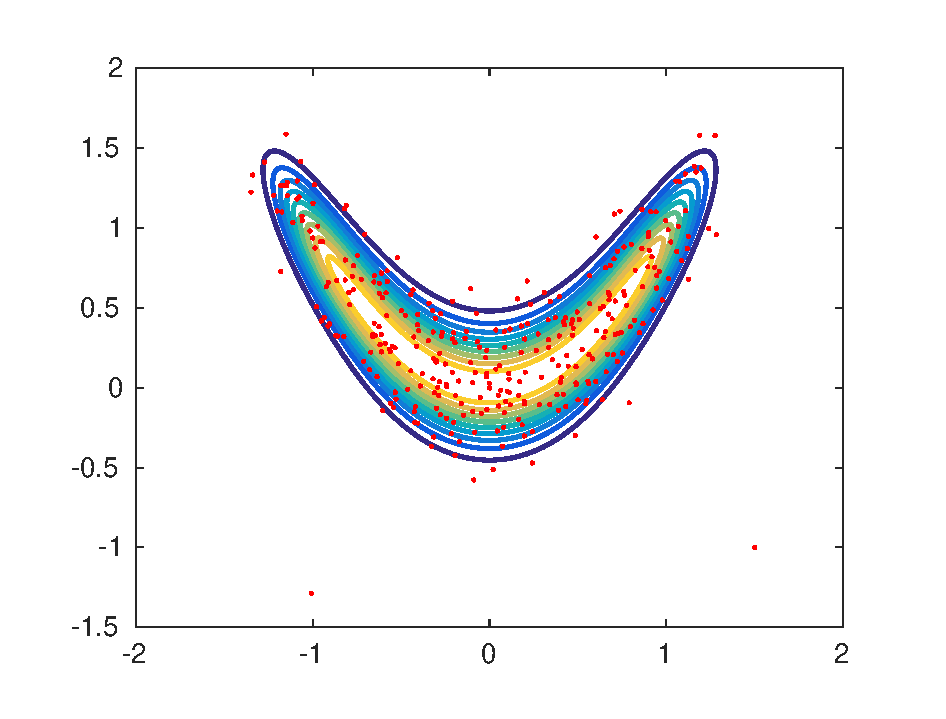
\includegraphics[width=1\linewidth]{plots/MHvsRAM/MH_big}
	\end{subfigure}
	\begin{subfigure}{0.32\linewidth}
		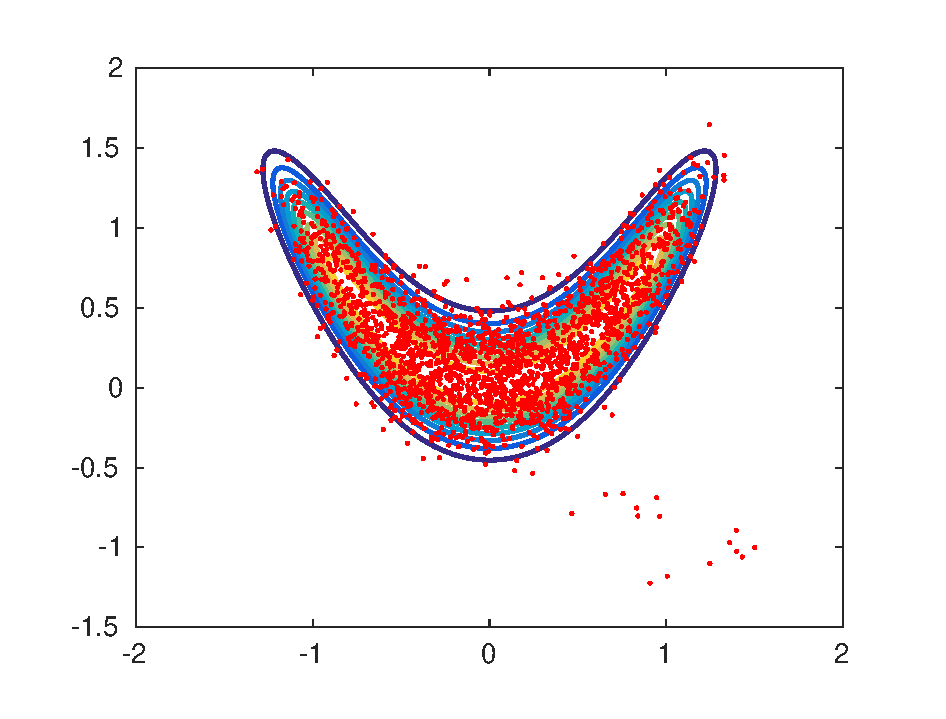
\includegraphics[width=1\linewidth]{plots/MHvsRAM/RAM_small}
	\end{subfigure}
	\begin{subfigure}{0.32\linewidth}
		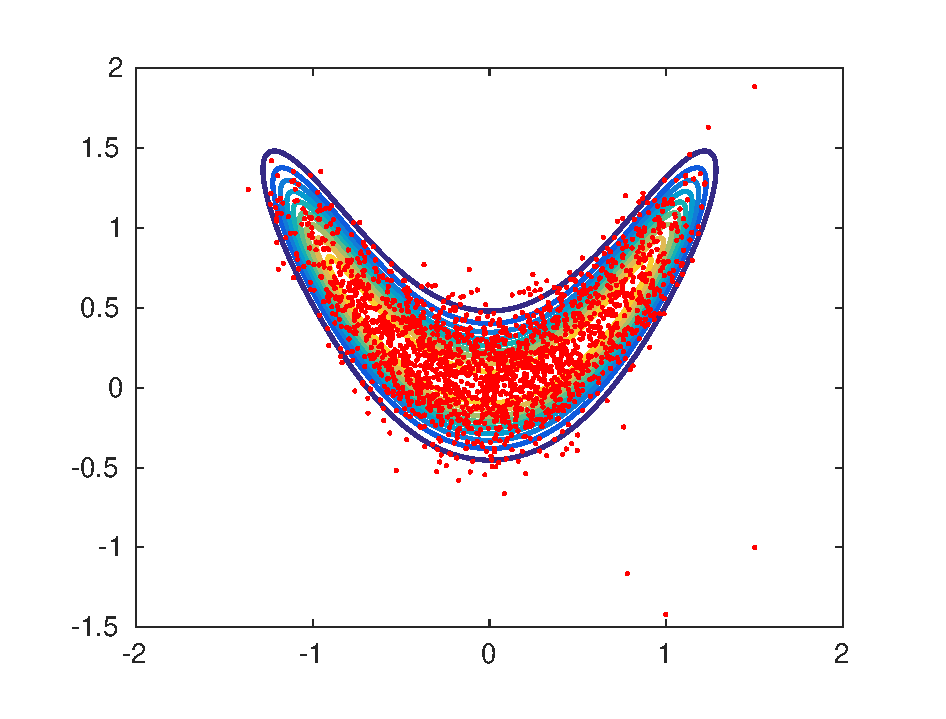
\includegraphics[width=1\linewidth]{plots/MHvsRAM/RAM_medium}
	\end{subfigure}
	\begin{subfigure}{0.32\linewidth}
		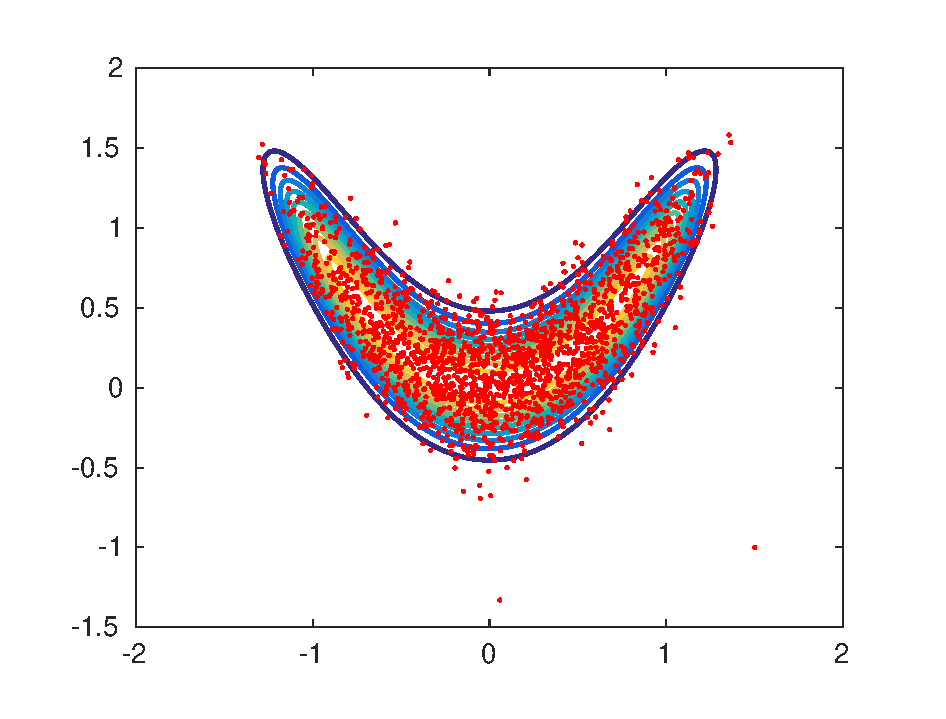
\includegraphics[width=1\linewidth]{plots/MHvsRAM/RAM_big}
	\end{subfigure}
	\caption{Samples produced by MH and RAM for the distribution \eqref{eq:RAMtestPi}. The contour lines of the density function are plotted for all the sets of results. In the first row we show the results obtained with MH for a normal update with covariance $\Sigma = \sigma^2 I $ with $\sigma = \{0.01, 0.5, 2.0\}$ from left to right. In the second row we show the results obtained with RAM with the same values of $\Sigma$ as an initial guess of the covariance structure. }
	\label{fig:RAMexample}
\end{figure}